\documentclass[1p]{elsarticle_modified}
%\bibliographystyle{elsarticle-num}

%\usepackage[colorlinks]{hyperref}
%\usepackage{abbrmath_seonhwa} %\Abb, \Ascr, \Acal ,\Abf, \Afrak
\usepackage{amsfonts}
\usepackage{amssymb}
\usepackage{amsmath}
\usepackage{amsthm}
\usepackage{scalefnt}
\usepackage{amsbsy}
\usepackage{kotex}
\usepackage{caption}
\usepackage{subfig}
\usepackage{color}
\usepackage{graphicx}
\usepackage{xcolor} %% white, black, red, green, blue, cyan, magenta, yellow
\usepackage{float}
\usepackage{setspace}
\usepackage{hyperref}

\usepackage{tikz}
\usetikzlibrary{arrows}

\usepackage{multirow}
\usepackage{array} % fixed length table
\usepackage{hhline}

%%%%%%%%%%%%%%%%%%%%%
\makeatletter
\renewcommand*\env@matrix[1][\arraystretch]{%
	\edef\arraystretch{#1}%
	\hskip -\arraycolsep
	\let\@ifnextchar\new@ifnextchar
	\array{*\c@MaxMatrixCols c}}
\makeatother %https://tex.stackexchange.com/questions/14071/how-can-i-increase-the-line-spacing-in-a-matrix
%%%%%%%%%%%%%%%

\usepackage[normalem]{ulem}

\newcommand{\msout}[1]{\ifmmode\text{\sout{\ensuremath{#1}}}\else\sout{#1}\fi}
%SOURCE: \msout is \stkout macro in https://tex.stackexchange.com/questions/20609/strikeout-in-math-mode

\newcommand{\cancel}[1]{
	\ifmmode
	{\color{red}\msout{#1}}
	\else
	{\color{red}\sout{#1}}
	\fi
}

\newcommand{\add}[1]{
	{\color{blue}\uwave{#1}}
}

\newcommand{\replace}[2]{
	\ifmmode
	{\color{red}\msout{#1}}{\color{blue}\uwave{#2}}
	\else
	{\color{red}\sout{#1}}{\color{blue}\uwave{#2}}
	\fi
}

\newcommand{\Sol}{\mathcal{S}} %segment
\newcommand{\D}{D} %diagram
\newcommand{\A}{\mathcal{A}} %arc


%%%%%%%%%%%%%%%%%%%%%%%%%%%%%5 test

\def\sl{\operatorname{\textup{SL}}(2,\Cbb)}
\def\psl{\operatorname{\textup{PSL}}(2,\Cbb)}
\def\quan{\mkern 1mu \triangleright \mkern 1mu}

\theoremstyle{definition}
\newtheorem{thm}{Theorem}[section]
\newtheorem{prop}[thm]{Proposition}
\newtheorem{lem}[thm]{Lemma}
\newtheorem{ques}[thm]{Question}
\newtheorem{cor}[thm]{Corollary}
\newtheorem{defn}[thm]{Definition}
\newtheorem{exam}[thm]{Example}
\newtheorem{rmk}[thm]{Remark}
\newtheorem{alg}[thm]{Algorithm}

\newcommand{\I}{\sqrt{-1}}
\begin{document}

%\begin{frontmatter}
%
%\title{Boundary parabolic representations of knots up to 8 crossings}
%
%%% Group authors per affiliation:
%\author{Yunhi Cho} 
%\address{Department of Mathematics, University of Seoul, Seoul, Korea}
%\ead{yhcho@uos.ac.kr}
%
%
%\author{Seonhwa Kim} %\fnref{s_kim}}
%\address{Center for Geometry and Physics, Institute for Basic Science, Pohang, 37673, Korea}
%\ead{ryeona17@ibs.re.kr}
%
%\author{Hyuk Kim}
%\address{Department of Mathematical Sciences, Seoul National University, Seoul 08826, Korea}
%\ead{hyukkim@snu.ac.kr}
%
%\author{Seokbeom Yoon}
%\address{Department of Mathematical Sciences, Seoul National University, Seoul, 08826,  Korea}
%\ead{sbyoon15@snu.ac.kr}
%
%\begin{abstract}
%We find all boundary parabolic representation of knots up to 8 crossings.
%
%\end{abstract}
%\begin{keyword}
%    \MSC[2010] 57M25 
%\end{keyword}
%
%\end{frontmatter}

%\linenumbers
%\tableofcontents
%
\newcommand\colored[1]{\textcolor{white}{\rule[-0.35ex]{0.8em}{1.4ex}}\kern-0.8em\color{red} #1}%
%\newcommand\colored[1]{\textcolor{white}{ #1}\kern-2.17ex	\textcolor{white}{ #1}\kern-1.81ex	\textcolor{white}{ #1}\kern-2.15ex\color{red}#1	}

{\Large $\underline{12a_{1235}~(K12a_{1235})}$}

\setlength{\tabcolsep}{10pt}
\renewcommand{\arraystretch}{1.6}
\vspace{1cm}\begin{tabular}{m{100pt}>{\centering\arraybackslash}m{274pt}}
\multirow{5}{120pt}{
	\centering
	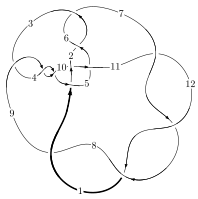
\includegraphics[width=112pt]{../../../GIT/diagram.site/Diagrams/png/2036_12a_1235.png}\\
\ \ \ A knot diagram\footnotemark}&
\allowdisplaybreaks
\textbf{Linearized knot diagam} \\
\cline{2-2}
 &
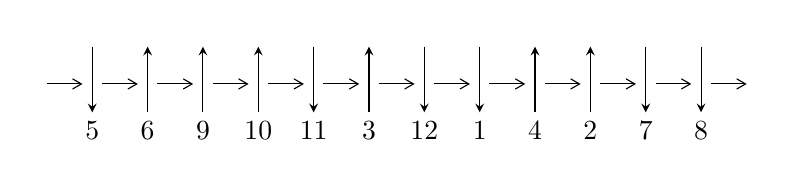
\begin{tikzpicture}[x=20pt, y=17pt]
	% nodes
	\node (C0) at (0, 0) {};
	\node (C1) at (1, 0) {};
	\node (C1U) at (1, +1) {};
	\node (C1D) at (1, -1) {5};

	\node (C2) at (2, 0) {};
	\node (C2U) at (2, +1) {};
	\node (C2D) at (2, -1) {6};

	\node (C3) at (3, 0) {};
	\node (C3U) at (3, +1) {};
	\node (C3D) at (3, -1) {9};

	\node (C4) at (4, 0) {};
	\node (C4U) at (4, +1) {};
	\node (C4D) at (4, -1) {10};

	\node (C5) at (5, 0) {};
	\node (C5U) at (5, +1) {};
	\node (C5D) at (5, -1) {11};

	\node (C6) at (6, 0) {};
	\node (C6U) at (6, +1) {};
	\node (C6D) at (6, -1) {3};

	\node (C7) at (7, 0) {};
	\node (C7U) at (7, +1) {};
	\node (C7D) at (7, -1) {12};

	\node (C8) at (8, 0) {};
	\node (C8U) at (8, +1) {};
	\node (C8D) at (8, -1) {1};

	\node (C9) at (9, 0) {};
	\node (C9U) at (9, +1) {};
	\node (C9D) at (9, -1) {4};

	\node (C10) at (10, 0) {};
	\node (C10U) at (10, +1) {};
	\node (C10D) at (10, -1) {2};

	\node (C11) at (11, 0) {};
	\node (C11U) at (11, +1) {};
	\node (C11D) at (11, -1) {7};

	\node (C12) at (12, 0) {};
	\node (C12U) at (12, +1) {};
	\node (C12D) at (12, -1) {8};
	\node (C13) at (13, 0) {};

	% arrows
	\draw[->,>={angle 60}]
	(C0) edge (C1) (C1) edge (C2) (C2) edge (C3) (C3) edge (C4) (C4) edge (C5) (C5) edge (C6) (C6) edge (C7) (C7) edge (C8) (C8) edge (C9) (C9) edge (C10) (C10) edge (C11) (C11) edge (C12) (C12) edge (C13) ;	\draw[->,>=stealth]
	(C1U) edge (C1D) (C2D) edge (C2U) (C3D) edge (C3U) (C4D) edge (C4U) (C5U) edge (C5D) (C6D) edge (C6U) (C7U) edge (C7D) (C8U) edge (C8D) (C9D) edge (C9U) (C10D) edge (C10U) (C11U) edge (C11D) (C12U) edge (C12D) ;
	\end{tikzpicture} \\
\hhline{~~} \\& 
\textbf{Solving Sequence} \\ \cline{2-2} 
 &
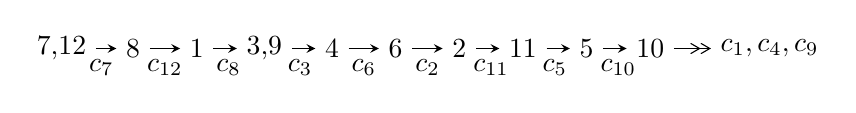
\begin{tikzpicture}[x=23pt, y=7pt]
	% node
	\node (A0) at (-1/8, 0) {7,12};
	\node (A1) at (1, 0) {8};
	\node (A2) at (2, 0) {1};
	\node (A3) at (49/16, 0) {3,9};
	\node (A4) at (33/8, 0) {4};
	\node (A5) at (41/8, 0) {6};
	\node (A6) at (49/8, 0) {2};
	\node (A7) at (57/8, 0) {11};
	\node (A8) at (65/8, 0) {5};
	\node (A9) at (73/8, 0) {10};
	\node (C1) at (1/2, -1) {$c_{7}$};
	\node (C2) at (3/2, -1) {$c_{12}$};
	\node (C3) at (5/2, -1) {$c_{8}$};
	\node (C4) at (29/8, -1) {$c_{3}$};
	\node (C5) at (37/8, -1) {$c_{6}$};
	\node (C6) at (45/8, -1) {$c_{2}$};
	\node (C7) at (53/8, -1) {$c_{11}$};
	\node (C8) at (61/8, -1) {$c_{5}$};
	\node (C9) at (69/8, -1) {$c_{10}$};
	\node (A10) at (11, 0) {$c_{1},c_{4},c_{9}$};

	% edge
	\draw[->,>=stealth]	
	(A0) edge (A1) (A1) edge (A2) (A2) edge (A3) (A3) edge (A4) (A4) edge (A5) (A5) edge (A6) (A6) edge (A7) (A7) edge (A8) (A8) edge (A9) ;
	\draw[->>,>={angle 60}]	
	(A9) edge (A10);
\end{tikzpicture} \\ 

\end{tabular} \\

\footnotetext{
The image of knot diagram is generated by the software ``\textbf{Draw programme}" developed by Andrew Bartholomew(\url{http://www.layer8.co.uk/maths/draw/index.htm\#Running-draw}), where we modified some parts for our purpose(\url{https://github.com/CATsTAILs/LinksPainter}).
}\phantom \\ \newline 
\centering \textbf{Ideals for irreducible components\footnotemark of $X_{\text{par}}$} 
 
\begin{align*}
I^u_{1}&=\langle 
-2.86883\times10^{97} u^{82}-1.55584\times10^{98} u^{81}+\cdots+7.14764\times10^{98} b-1.16306\times10^{99},\\
\phantom{I^u_{1}}&\phantom{= \langle  }-1.14478\times10^{98} u^{82}-2.39182\times10^{98} u^{81}+\cdots+7.14764\times10^{98} a-3.16119\times10^{99},\;u^{83}+u^{82}+\cdots+9 u-1\rangle \\
I^u_{2}&=\langle 
- u^{14}+10 u^{12}+u^{11}-39 u^{10}-8 u^9+75 u^8+23 u^7-74 u^6-29 u^5+35 u^4+17 u^3-6 u^2+b-5 u+1,\\
\phantom{I^u_{2}}&\phantom{= \langle  }u^{15}- u^{14}+\cdots+a-1,\;u^{17}-12 u^{15}+\cdots+2 u+1\rangle \\
\\
\end{align*}
\raggedright * 2 irreducible components of $\dim_{\mathbb{C}}=0$, with total 100 representations.\\
\footnotetext{All coefficients of polynomials are rational numbers. But the coefficients are sometimes approximated in decimal forms when there is not enough margin.}
\newpage
\renewcommand{\arraystretch}{1}
\centering \section*{I. $I^u_{1}= \langle -2.87\times10^{97} u^{82}-1.56\times10^{98} u^{81}+\cdots+7.15\times10^{98} b-1.16\times10^{99},\;-1.14\times10^{98} u^{82}-2.39\times10^{98} u^{81}+\cdots+7.15\times10^{98} a-3.16\times10^{99},\;u^{83}+u^{82}+\cdots+9 u-1 \rangle$}
\flushleft \textbf{(i) Arc colorings}\\
\begin{tabular}{m{7pt} m{180pt} m{7pt} m{180pt} }
\flushright $a_{7}=$&$\begin{pmatrix}1\\0\end{pmatrix}$ \\
\flushright $a_{12}=$&$\begin{pmatrix}0\\u\end{pmatrix}$ \\
\flushright $a_{8}=$&$\begin{pmatrix}1\\u^2\end{pmatrix}$ \\
\flushright $a_{1}=$&$\begin{pmatrix}- u\\- u^3+u\end{pmatrix}$ \\
\flushright $a_{3}=$&$\begin{pmatrix}0.160162 u^{82}+0.334631 u^{81}+\cdots-0.747532 u+4.42271\\0.0401367 u^{82}+0.217672 u^{81}+\cdots+0.925102 u+1.62720\end{pmatrix}$ \\
\flushright $a_{9}=$&$\begin{pmatrix}- u^2+1\\- u^4+2 u^2\end{pmatrix}$ \\
\flushright $a_{4}=$&$\begin{pmatrix}0.213196 u^{82}+0.466612 u^{81}+\cdots+0.0323716 u+5.97524\\0.00962191 u^{82}+0.239696 u^{81}+\cdots+0.902950 u+1.65279\end{pmatrix}$ \\
\flushright $a_{6}=$&$\begin{pmatrix}0.428885 u^{82}+0.918419 u^{81}+\cdots+1.55236 u+8.53499\\0.0169089 u^{82}+0.434079 u^{81}+\cdots-0.349604 u+3.04904\end{pmatrix}$ \\
\flushright $a_{2}=$&$\begin{pmatrix}-0.826939 u^{82}-1.72921 u^{81}+\cdots-4.55454 u-10.5230\\0.0411460 u^{82}-0.623126 u^{81}+\cdots+2.08602 u-3.87008\end{pmatrix}$ \\
\flushright $a_{11}=$&$\begin{pmatrix}u\\u\end{pmatrix}$ \\
\flushright $a_{5}=$&$\begin{pmatrix}0.428878 u^{82}+0.873387 u^{81}+\cdots+1.79165 u+8.46262\\0.0169013 u^{82}+0.389047 u^{81}+\cdots-0.110312 u+2.97668\end{pmatrix}$ \\
\flushright $a_{10}=$&$\begin{pmatrix}-0.958590 u^{82}-0.625662 u^{81}+\cdots-3.45210 u-8.51747\\-0.504620 u^{82}-0.211045 u^{81}+\cdots-2.58924 u-2.59056\end{pmatrix}$\\&\end{tabular}
\flushleft \textbf{(ii) Obstruction class $= -1$}\\~\\
\flushleft \textbf{(iii) Cusp Shapes $= 1.80406 u^{82}+2.42592 u^{81}+\cdots+2.92566 u+25.5968$}\\~\\
\newpage\renewcommand{\arraystretch}{1}
\flushleft \textbf{(iv) u-Polynomials at the component}\newline \\
\begin{tabular}{m{50pt}|m{274pt}}
Crossings & \hspace{64pt}u-Polynomials at each crossing \\
\hline $$\begin{aligned}c_{1}\end{aligned}$$&$\begin{aligned}
&u^{83}+5 u^{82}+\cdots+719 u-479
\end{aligned}$\\
\hline $$\begin{aligned}c_{2},c_{6}\end{aligned}$$&$\begin{aligned}
&u^{83}-28 u^{81}+\cdots-22 u-73
\end{aligned}$\\
\hline $$\begin{aligned}c_{3},c_{4},c_{9}\end{aligned}$$&$\begin{aligned}
&u^{83}- u^{82}+\cdots-4 u+8
\end{aligned}$\\
\hline $$\begin{aligned}c_{5}\end{aligned}$$&$\begin{aligned}
&u^{83}+u^{82}+\cdots+34 u-1
\end{aligned}$\\
\hline $$\begin{aligned}c_{7},c_{8},c_{11}\\c_{12}\end{aligned}$$&$\begin{aligned}
&u^{83}- u^{82}+\cdots+9 u+1
\end{aligned}$\\
\hline $$\begin{aligned}c_{10}\end{aligned}$$&$\begin{aligned}
&u^{83}-2 u^{82}+\cdots+736 u+1561
\end{aligned}$\\
\hline
\end{tabular}\\~\\
\newpage\renewcommand{\arraystretch}{1}
\flushleft \textbf{(v) Riley Polynomials at the component}\newline \\
\begin{tabular}{m{50pt}|m{274pt}}
Crossings & \hspace{64pt}Riley Polynomials at each crossing \\
\hline $$\begin{aligned}c_{1}\end{aligned}$$&$\begin{aligned}
&y^{83}+9 y^{82}+\cdots+384757 y-229441
\end{aligned}$\\
\hline $$\begin{aligned}c_{2},c_{6}\end{aligned}$$&$\begin{aligned}
&y^{83}-56 y^{82}+\cdots+97428 y-5329
\end{aligned}$\\
\hline $$\begin{aligned}c_{3},c_{4},c_{9}\end{aligned}$$&$\begin{aligned}
&y^{83}-83 y^{82}+\cdots-304 y-64
\end{aligned}$\\
\hline $$\begin{aligned}c_{5}\end{aligned}$$&$\begin{aligned}
&y^{83}+y^{82}+\cdots+750 y-1
\end{aligned}$\\
\hline $$\begin{aligned}c_{7},c_{8},c_{11}\\c_{12}\end{aligned}$$&$\begin{aligned}
&y^{83}-99 y^{82}+\cdots+83 y-1
\end{aligned}$\\
\hline $$\begin{aligned}c_{10}\end{aligned}$$&$\begin{aligned}
&y^{83}-34 y^{82}+\cdots+95556644 y-2436721
\end{aligned}$\\
\hline
\end{tabular}\\~\\
\newpage\flushleft \textbf{(vi) Complex Volumes and Cusp Shapes}
$$\begin{array}{c|c|c}  
\text{Solutions to }I^u_{1}& \I (\text{vol} + \sqrt{-1}CS) & \text{Cusp shape}\\
 \hline 
\begin{aligned}
u &= \phantom{-}0.768082 + 0.691197 I \\
a &= \phantom{-}0.252642 + 1.292600 I \\
b &= -1.33555 + 0.56553 I\end{aligned}
 & \phantom{-}7.6353 - 12.3651 I & \phantom{-0.000000 } 0 \\ \hline\begin{aligned}
u &= \phantom{-}0.768082 - 0.691197 I \\
a &= \phantom{-}0.252642 - 1.292600 I \\
b &= -1.33555 - 0.56553 I\end{aligned}
 & \phantom{-}7.6353 + 12.3651 I & \phantom{-0.000000 } 0 \\ \hline\begin{aligned}
u &= -0.866895 + 0.373017 I \\
a &= \phantom{-}0.922412 - 0.077651 I \\
b &= -0.597906 - 0.120958 I\end{aligned}
 & \phantom{-}2.82259 - 0.53209 I & \phantom{-0.000000 } 0 \\ \hline\begin{aligned}
u &= -0.866895 - 0.373017 I \\
a &= \phantom{-}0.922412 + 0.077651 I \\
b &= -0.597906 + 0.120958 I\end{aligned}
 & \phantom{-}2.82259 + 0.53209 I & \phantom{-0.000000 } 0 \\ \hline\begin{aligned}
u &= \phantom{-}0.235435 + 0.882232 I \\
a &= \phantom{-}0.296158 + 0.219377 I \\
b &= -1.254670 - 0.403627 I\end{aligned}
 & \phantom{-}9.25233 + 7.20437 I & \phantom{-0.000000 } 0 \\ \hline\begin{aligned}
u &= \phantom{-}0.235435 - 0.882232 I \\
a &= \phantom{-}0.296158 - 0.219377 I \\
b &= -1.254670 + 0.403627 I\end{aligned}
 & \phantom{-}9.25233 - 7.20437 I & \phantom{-0.000000 } 0 \\ \hline\begin{aligned}
u &= -0.731931 + 0.526717 I \\
a &= -0.55919 + 1.43057 I \\
b &= \phantom{-}1.251280 + 0.487251 I\end{aligned}
 & \phantom{-}1.12377 + 8.38932 I & \phantom{-0.000000 } 0 \\ \hline\begin{aligned}
u &= -0.731931 - 0.526717 I \\
a &= -0.55919 - 1.43057 I \\
b &= \phantom{-}1.251280 - 0.487251 I\end{aligned}
 & \phantom{-}1.12377 - 8.38932 I & \phantom{-0.000000 } 0 \\ \hline\begin{aligned}
u &= -0.502172 + 0.729866 I \\
a &= \phantom{-}0.808477 - 1.017140 I \\
b &= -0.836691 - 0.506283 I\end{aligned}
 & \phantom{-}3.26194 + 4.42234 I & \phantom{-0.000000 } 0 \\ \hline\begin{aligned}
u &= -0.502172 - 0.729866 I \\
a &= \phantom{-}0.808477 + 1.017140 I \\
b &= -0.836691 + 0.506283 I\end{aligned}
 & \phantom{-}3.26194 - 4.42234 I & \phantom{-0.000000 } 0\\
 \hline 
 \end{array}$$\newpage$$\begin{array}{c|c|c}  
\text{Solutions to }I^u_{1}& \I (\text{vol} + \sqrt{-1}CS) & \text{Cusp shape}\\
 \hline 
\begin{aligned}
u &= -0.741521 + 0.479666 I \\
a &= \phantom{-}0.61796 + 1.69432 I \\
b &= \phantom{-}1.180280 + 0.049298 I\end{aligned}
 & \phantom{-}7.90154 + 3.78747 I & \phantom{-0.000000 } 0 \\ \hline\begin{aligned}
u &= -0.741521 - 0.479666 I \\
a &= \phantom{-}0.61796 - 1.69432 I \\
b &= \phantom{-}1.180280 - 0.049298 I\end{aligned}
 & \phantom{-}7.90154 - 3.78747 I & \phantom{-0.000000 } 0 \\ \hline\begin{aligned}
u &= \phantom{-}0.759993 + 0.438039 I \\
a &= \phantom{-}0.51802 - 1.64118 I \\
b &= \phantom{-}1.39103 - 0.62751 I\end{aligned}
 & \phantom{-}7.59156 - 2.88645 I & \phantom{-0.000000 } 0 \\ \hline\begin{aligned}
u &= \phantom{-}0.759993 - 0.438039 I \\
a &= \phantom{-}0.51802 + 1.64118 I \\
b &= \phantom{-}1.39103 + 0.62751 I\end{aligned}
 & \phantom{-}7.59156 + 2.88645 I & \phantom{-0.000000 } 0 \\ \hline\begin{aligned}
u &= \phantom{-}1.065910 + 0.374554 I \\
a &= \phantom{-}0.230666 - 0.271570 I \\
b &= \phantom{-}0.886114 + 0.262946 I\end{aligned}
 & -0.720339 + 0.792513 I & \phantom{-0.000000 } 0 \\ \hline\begin{aligned}
u &= \phantom{-}1.065910 - 0.374554 I \\
a &= \phantom{-}0.230666 + 0.271570 I \\
b &= \phantom{-}0.886114 - 0.262946 I\end{aligned}
 & -0.720339 - 0.792513 I & \phantom{-0.000000 } 0 \\ \hline\begin{aligned}
u &= \phantom{-}0.835796 + 0.060616 I \\
a &= -0.741566 - 0.326162 I \\
b &= -0.139599 - 0.295553 I\end{aligned}
 & -1.73821 - 0.12176 I & \phantom{-0.000000 } 0 \\ \hline\begin{aligned}
u &= \phantom{-}0.835796 - 0.060616 I \\
a &= -0.741566 + 0.326162 I \\
b &= -0.139599 + 0.295553 I\end{aligned}
 & -1.73821 + 0.12176 I & \phantom{-0.000000 } 0 \\ \hline\begin{aligned}
u &= -0.605321 + 0.578215 I \\
a &= \phantom{-}0.022688 + 0.194967 I \\
b &= -0.662120 + 0.544490 I\end{aligned}
 & \phantom{-}2.82569 + 0.10655 I & \phantom{-0.000000 } 0 \\ \hline\begin{aligned}
u &= -0.605321 - 0.578215 I \\
a &= \phantom{-}0.022688 - 0.194967 I \\
b &= -0.662120 - 0.544490 I\end{aligned}
 & \phantom{-}2.82569 - 0.10655 I & \phantom{-0.000000 } 0\\
 \hline 
 \end{array}$$\newpage$$\begin{array}{c|c|c}  
\text{Solutions to }I^u_{1}& \I (\text{vol} + \sqrt{-1}CS) & \text{Cusp shape}\\
 \hline 
\begin{aligned}
u &= -0.774756 + 0.279655 I \\
a &= \phantom{-}0.409521 - 0.846501 I \\
b &= \phantom{-}0.075986 - 0.890444 I\end{aligned}
 & -2.46982 + 3.44779 I & \phantom{-0.000000 } 0 \\ \hline\begin{aligned}
u &= -0.774756 - 0.279655 I \\
a &= \phantom{-}0.409521 + 0.846501 I \\
b &= \phantom{-}0.075986 + 0.890444 I\end{aligned}
 & -2.46982 - 3.44779 I & \phantom{-0.000000 } 0 \\ \hline\begin{aligned}
u &= \phantom{-}0.598146 + 0.543807 I \\
a &= -0.747680 - 0.822006 I \\
b &= \phantom{-}0.797769 - 0.293360 I\end{aligned}
 & -0.78891 - 1.85485 I & \phantom{-0.000000 } 0 \\ \hline\begin{aligned}
u &= \phantom{-}0.598146 - 0.543807 I \\
a &= -0.747680 + 0.822006 I \\
b &= \phantom{-}0.797769 + 0.293360 I\end{aligned}
 & -0.78891 + 1.85485 I & \phantom{-0.000000 } 0 \\ \hline\begin{aligned}
u &= \phantom{-}0.666365 + 0.433298 I \\
a &= -0.252771 - 1.104390 I \\
b &= -0.032199 - 1.198920 I\end{aligned}
 & \phantom{-}3.54914 - 6.33411 I & \phantom{-0.000000 -}0. + 8.16822 I \\ \hline\begin{aligned}
u &= \phantom{-}0.666365 - 0.433298 I \\
a &= -0.252771 + 1.104390 I \\
b &= -0.032199 + 1.198920 I\end{aligned}
 & \phantom{-}3.54914 + 6.33411 I & \phantom{-0.000000 } 0. - 8.16822 I \\ \hline\begin{aligned}
u &= -0.137211 + 0.664955 I \\
a &= -1.008040 + 0.313227 I \\
b &= \phantom{-}1.111180 - 0.371677 I\end{aligned}
 & \phantom{-}2.87567 - 4.41134 I & \phantom{-}3.53322 + 5.88957 I \\ \hline\begin{aligned}
u &= -0.137211 - 0.664955 I \\
a &= -1.008040 - 0.313227 I \\
b &= \phantom{-}1.111180 + 0.371677 I\end{aligned}
 & \phantom{-}2.87567 + 4.41134 I & \phantom{-}3.53322 - 5.88957 I \\ \hline\begin{aligned}
u &= \phantom{-}0.555148 + 0.350297 I \\
a &= \phantom{-}1.40971 + 1.37443 I \\
b &= -1.219220 + 0.311712 I\end{aligned}
 & \phantom{-}1.52584 - 2.93851 I & \phantom{-}2.21348 + 8.51205 I \\ \hline\begin{aligned}
u &= \phantom{-}0.555148 - 0.350297 I \\
a &= \phantom{-}1.40971 - 1.37443 I \\
b &= -1.219220 - 0.311712 I\end{aligned}
 & \phantom{-}1.52584 + 2.93851 I & \phantom{-}2.21348 - 8.51205 I\\
 \hline 
 \end{array}$$\newpage$$\begin{array}{c|c|c}  
\text{Solutions to }I^u_{1}& \I (\text{vol} + \sqrt{-1}CS) & \text{Cusp shape}\\
 \hline 
\begin{aligned}
u &= -1.284960 + 0.532591 I \\
a &= -0.606372 - 0.317238 I \\
b &= -1.101640 + 0.237984 I\end{aligned}
 & \phantom{-}4.61964 - 2.27072 I & \phantom{-0.000000 } 0 \\ \hline\begin{aligned}
u &= -1.284960 - 0.532591 I \\
a &= -0.606372 + 0.317238 I \\
b &= -1.101640 - 0.237984 I\end{aligned}
 & \phantom{-}4.61964 + 2.27072 I & \phantom{-0.000000 } 0 \\ \hline\begin{aligned}
u &= -0.499318 + 0.304404 I \\
a &= \phantom{-}0.15040 - 2.11729 I \\
b &= -1.091140 - 0.571643 I\end{aligned}
 & \phantom{-}1.74936 + 2.54506 I & \phantom{-}4.42588 - 10.86296 I \\ \hline\begin{aligned}
u &= -0.499318 - 0.304404 I \\
a &= \phantom{-}0.15040 + 2.11729 I \\
b &= -1.091140 + 0.571643 I\end{aligned}
 & \phantom{-}1.74936 - 2.54506 I & \phantom{-}4.42588 + 10.86296 I \\ \hline\begin{aligned}
u &= \phantom{-}0.452167 + 0.325212 I \\
a &= \phantom{-}0.58482 + 2.60510 I \\
b &= -1.002000 - 0.101348 I\end{aligned}
 & \phantom{-}1.85705 + 0.45025 I & \phantom{-}3.87420 + 1.56486 I \\ \hline\begin{aligned}
u &= \phantom{-}0.452167 - 0.325212 I \\
a &= \phantom{-}0.58482 - 2.60510 I \\
b &= -1.002000 + 0.101348 I\end{aligned}
 & \phantom{-}1.85705 - 0.45025 I & \phantom{-}3.87420 - 1.56486 I \\ \hline\begin{aligned}
u &= -0.054260 + 0.528821 I \\
a &= -0.542993 - 0.539629 I \\
b &= \phantom{-}1.44268 + 0.17108 I\end{aligned}
 & \phantom{-}9.81715 - 0.31683 I & \phantom{-}9.58825 - 0.96575 I \\ \hline\begin{aligned}
u &= -0.054260 - 0.528821 I \\
a &= -0.542993 + 0.539629 I \\
b &= \phantom{-}1.44268 - 0.17108 I\end{aligned}
 & \phantom{-}9.81715 + 0.31683 I & \phantom{-}9.58825 + 0.96575 I \\ \hline\begin{aligned}
u &= \phantom{-}1.49008\phantom{ +0.000000I} \\
a &= \phantom{-}0.452163\phantom{ +0.000000I} \\
b &= \phantom{-}1.68796\phantom{ +0.000000I}\end{aligned}
 & \phantom{-}4.72540\phantom{ +0.000000I} & \phantom{-0.000000 } 0 \\ \hline\begin{aligned}
u &= \phantom{-}1.49221 + 0.03214 I \\
a &= -0.02163 + 1.51967 I \\
b &= \phantom{-}0.808869 + 0.200589 I\end{aligned}
 & -0.82324 - 4.29800 I & \phantom{-0.000000 } 0\\
 \hline 
 \end{array}$$\newpage$$\begin{array}{c|c|c}  
\text{Solutions to }I^u_{1}& \I (\text{vol} + \sqrt{-1}CS) & \text{Cusp shape}\\
 \hline 
\begin{aligned}
u &= \phantom{-}1.49221 - 0.03214 I \\
a &= -0.02163 - 1.51967 I \\
b &= \phantom{-}0.808869 - 0.200589 I\end{aligned}
 & -0.82324 + 4.29800 I & \phantom{-0.000000 } 0 \\ \hline\begin{aligned}
u &= -0.420439 + 0.274945 I \\
a &= -0.115243 - 0.576490 I \\
b &= -1.037550 + 0.209794 I\end{aligned}
 & \phantom{-}1.89083 - 0.25563 I & \phantom{-}4.66041 - 1.63586 I \\ \hline\begin{aligned}
u &= -0.420439 - 0.274945 I \\
a &= -0.115243 + 0.576490 I \\
b &= -1.037550 - 0.209794 I\end{aligned}
 & \phantom{-}1.89083 + 0.25563 I & \phantom{-}4.66041 + 1.63586 I \\ \hline\begin{aligned}
u &= -1.50758 + 0.03846 I \\
a &= \phantom{-}0.68100 - 1.96909 I \\
b &= \phantom{-}0.998445 - 0.934747 I\end{aligned}
 & -1.10641 - 2.50144 I & \phantom{-0.000000 } 0 \\ \hline\begin{aligned}
u &= -1.50758 - 0.03846 I \\
a &= \phantom{-}0.68100 + 1.96909 I \\
b &= \phantom{-}0.998445 + 0.934747 I\end{aligned}
 & -1.10641 + 2.50144 I & \phantom{-0.000000 } 0 \\ \hline\begin{aligned}
u &= -1.51416\phantom{ +0.000000I} \\
a &= \phantom{-}1.76375\phantom{ +0.000000I} \\
b &= \phantom{-}2.20627\phantom{ +0.000000I}\end{aligned}
 & \phantom{-}4.11044\phantom{ +0.000000I} & \phantom{-0.000000 } 0 \\ \hline\begin{aligned}
u &= -1.54919 + 0.07124 I \\
a &= -0.47695 - 1.54171 I \\
b &= -0.924141 - 0.190121 I\end{aligned}
 & -5.00465 + 0.83960 I & \phantom{-0.000000 } 0 \\ \hline\begin{aligned}
u &= -1.54919 - 0.07124 I \\
a &= -0.47695 + 1.54171 I \\
b &= -0.924141 + 0.190121 I\end{aligned}
 & -5.00465 - 0.83960 I & \phantom{-0.000000 } 0 \\ \hline\begin{aligned}
u &= \phantom{-}1.56347 + 0.06819 I \\
a &= -0.78560 + 1.75556 I \\
b &= -1.14540 + 0.90049 I\end{aligned}
 & -5.34195 - 3.77537 I & \phantom{-0.000000 } 0 \\ \hline\begin{aligned}
u &= \phantom{-}1.56347 - 0.06819 I \\
a &= -0.78560 - 1.75556 I \\
b &= -1.14540 - 0.90049 I\end{aligned}
 & -5.34195 + 3.77537 I & \phantom{-0.000000 } 0\\
 \hline 
 \end{array}$$\newpage$$\begin{array}{c|c|c}  
\text{Solutions to }I^u_{1}& \I (\text{vol} + \sqrt{-1}CS) & \text{Cusp shape}\\
 \hline 
\begin{aligned}
u &= -1.57107 + 0.09416 I \\
a &= -0.166949 - 1.254180 I \\
b &= -1.38879 - 0.41637 I\end{aligned}
 & -5.75176 + 4.51699 I & \phantom{-0.000000 } 0 \\ \hline\begin{aligned}
u &= -1.57107 - 0.09416 I \\
a &= -0.166949 + 1.254180 I \\
b &= -1.38879 + 0.41637 I\end{aligned}
 & -5.75176 - 4.51699 I & \phantom{-0.000000 } 0 \\ \hline\begin{aligned}
u &= \phantom{-}1.55834 + 0.24296 I \\
a &= -0.02366 + 1.51038 I \\
b &= -0.963467 + 0.634147 I\end{aligned}
 & -3.58166 - 8.00557 I & \phantom{-0.000000 } 0 \\ \hline\begin{aligned}
u &= \phantom{-}1.55834 - 0.24296 I \\
a &= -0.02366 - 1.51038 I \\
b &= -0.963467 - 0.634147 I\end{aligned}
 & -3.58166 + 8.00557 I & \phantom{-0.000000 } 0 \\ \hline\begin{aligned}
u &= \phantom{-}1.57285 + 0.14448 I \\
a &= -0.592693 - 1.011330 I \\
b &= -0.679658 - 0.812394 I\end{aligned}
 & -4.48210 - 2.61438 I & \phantom{-0.000000 } 0 \\ \hline\begin{aligned}
u &= \phantom{-}1.57285 - 0.14448 I \\
a &= -0.592693 + 1.011330 I \\
b &= -0.679658 + 0.812394 I\end{aligned}
 & -4.48210 + 2.61438 I & \phantom{-0.000000 } 0 \\ \hline\begin{aligned}
u &= \phantom{-}0.085058 + 0.399319 I \\
a &= -0.716080 - 0.440615 I \\
b &= \phantom{-}0.043328 + 0.425943 I\end{aligned}
 & \phantom{-}0.023615 - 1.107130 I & \phantom{-}0.24981 + 5.47165 I \\ \hline\begin{aligned}
u &= \phantom{-}0.085058 - 0.399319 I \\
a &= -0.716080 + 0.440615 I \\
b &= \phantom{-}0.043328 - 0.425943 I\end{aligned}
 & \phantom{-}0.023615 + 1.107130 I & \phantom{-}0.24981 - 5.47165 I \\ \hline\begin{aligned}
u &= -1.58914 + 0.16134 I \\
a &= \phantom{-}0.135384 + 1.207830 I \\
b &= \phantom{-}1.053060 + 0.533761 I\end{aligned}
 & -8.22990 + 4.45911 I & \phantom{-0.000000 } 0 \\ \hline\begin{aligned}
u &= -1.58914 - 0.16134 I \\
a &= \phantom{-}0.135384 - 1.207830 I \\
b &= \phantom{-}1.053060 - 0.533761 I\end{aligned}
 & -8.22990 - 4.45911 I & \phantom{-0.000000 } 0\\
 \hline 
 \end{array}$$\newpage$$\begin{array}{c|c|c}  
\text{Solutions to }I^u_{1}& \I (\text{vol} + \sqrt{-1}CS) & \text{Cusp shape}\\
 \hline 
\begin{aligned}
u &= \phantom{-}1.59660 + 0.07112 I \\
a &= -0.407344 + 0.653461 I \\
b &= -1.263460 + 0.332042 I\end{aligned}
 & -5.48564 - 0.54881 I & \phantom{-0.000000 } 0 \\ \hline\begin{aligned}
u &= \phantom{-}1.59660 - 0.07112 I \\
a &= -0.407344 - 0.653461 I \\
b &= -1.263460 - 0.332042 I\end{aligned}
 & -5.48564 + 0.54881 I & \phantom{-0.000000 } 0 \\ \hline\begin{aligned}
u &= -1.59450 + 0.12611 I \\
a &= -0.39069 + 1.82656 I \\
b &= -0.22128 + 1.47922 I\end{aligned}
 & -4.13693 + 8.41109 I & \phantom{-0.000000 } 0 \\ \hline\begin{aligned}
u &= -1.59450 - 0.12611 I \\
a &= -0.39069 - 1.82656 I \\
b &= -0.22128 - 1.47922 I\end{aligned}
 & -4.13693 - 8.41109 I & \phantom{-0.000000 } 0 \\ \hline\begin{aligned}
u &= \phantom{-}0.201705 + 0.326921 I \\
a &= \phantom{-}2.77973 + 1.57851 I \\
b &= \phantom{-}0.449464 + 0.725917 I\end{aligned}
 & \phantom{-}4.91629 + 3.36888 I & \phantom{-}3.38585 - 1.71367 I \\ \hline\begin{aligned}
u &= \phantom{-}0.201705 - 0.326921 I \\
a &= \phantom{-}2.77973 - 1.57851 I \\
b &= \phantom{-}0.449464 - 0.725917 I\end{aligned}
 & \phantom{-}4.91629 - 3.36888 I & \phantom{-}3.38585 + 1.71367 I \\ \hline\begin{aligned}
u &= \phantom{-}1.61261 + 0.15634 I \\
a &= \phantom{-}0.39427 - 1.52840 I \\
b &= \phantom{-}1.35704 - 0.60605 I\end{aligned}
 & -6.81274 - 10.95820 I & \phantom{-0.000000 } 0 \\ \hline\begin{aligned}
u &= \phantom{-}1.61261 - 0.15634 I \\
a &= \phantom{-}0.39427 + 1.52840 I \\
b &= \phantom{-}1.35704 + 0.60605 I\end{aligned}
 & -6.81274 + 10.95820 I & \phantom{-0.000000 } 0 \\ \hline\begin{aligned}
u &= \phantom{-}1.61775 + 0.14984 I \\
a &= \phantom{-}0.88961 - 1.28448 I \\
b &= \phantom{-}0.998630 - 0.221072 I\end{aligned}
 & -0.12435 - 6.19456 I & \phantom{-0.000000 } 0 \\ \hline\begin{aligned}
u &= \phantom{-}1.61775 - 0.14984 I \\
a &= \phantom{-}0.88961 + 1.28448 I \\
b &= \phantom{-}0.998630 + 0.221072 I\end{aligned}
 & -0.12435 + 6.19456 I & \phantom{-0.000000 } 0\\
 \hline 
 \end{array}$$\newpage$$\begin{array}{c|c|c}  
\text{Solutions to }I^u_{1}& \I (\text{vol} + \sqrt{-1}CS) & \text{Cusp shape}\\
 \hline 
\begin{aligned}
u &= \phantom{-}1.62616 + 0.06822 I \\
a &= \phantom{-}0.30884 + 1.49012 I \\
b &= \phantom{-}0.105281 + 1.165260 I\end{aligned}
 & -10.74930 - 4.72000 I & \phantom{-0.000000 } 0 \\ \hline\begin{aligned}
u &= \phantom{-}1.62616 - 0.06822 I \\
a &= \phantom{-}0.30884 - 1.49012 I \\
b &= \phantom{-}0.105281 - 1.165260 I\end{aligned}
 & -10.74930 + 4.72000 I & \phantom{-0.000000 } 0 \\ \hline\begin{aligned}
u &= -1.62426 + 0.13524 I \\
a &= \phantom{-}0.97669 + 1.71202 I \\
b &= \phantom{-}1.25823 + 0.93663 I\end{aligned}
 & -0.55167 + 5.09041 I & \phantom{-0.000000 } 0 \\ \hline\begin{aligned}
u &= -1.62426 - 0.13524 I \\
a &= \phantom{-}0.97669 - 1.71202 I \\
b &= \phantom{-}1.25823 - 0.93663 I\end{aligned}
 & -0.55167 - 5.09041 I & \phantom{-0.000000 } 0 \\ \hline\begin{aligned}
u &= -1.62996 + 0.21685 I \\
a &= -0.53811 - 1.61542 I \\
b &= -1.38415 - 0.71622 I\end{aligned}
 & -0.3993 + 15.8170 I & \phantom{-0.000000 } 0 \\ \hline\begin{aligned}
u &= -1.62996 - 0.21685 I \\
a &= -0.53811 + 1.61542 I \\
b &= -1.38415 + 0.71622 I\end{aligned}
 & -0.3993 - 15.8170 I & \phantom{-0.000000 } 0 \\ \hline\begin{aligned}
u &= -0.132784 + 0.329558 I \\
a &= \phantom{-}2.33743 - 2.97261 I \\
b &= \phantom{-}0.332026 + 0.247657 I\end{aligned}
 & \phantom{-}4.91640 + 3.48534 I & \phantom{-}6.06358 - 0.28376 I \\ \hline\begin{aligned}
u &= -0.132784 - 0.329558 I \\
a &= \phantom{-}2.33743 + 2.97261 I \\
b &= \phantom{-}0.332026 - 0.247657 I\end{aligned}
 & \phantom{-}4.91640 - 3.48534 I & \phantom{-}6.06358 + 0.28376 I \\ \hline\begin{aligned}
u &= -1.64700 + 0.01472 I \\
a &= -0.044159 - 0.956622 I \\
b &= \phantom{-}0.183647 - 0.730460 I\end{aligned}
 & -10.48590 - 0.17400 I & \phantom{-0.000000 } 0 \\ \hline\begin{aligned}
u &= -1.64700 - 0.01472 I \\
a &= -0.044159 + 0.956622 I \\
b &= \phantom{-}0.183647 + 0.730460 I\end{aligned}
 & -10.48590 + 0.17400 I & \phantom{-0.000000 } 0\\
 \hline 
 \end{array}$$\newpage$$\begin{array}{c|c|c}  
\text{Solutions to }I^u_{1}& \I (\text{vol} + \sqrt{-1}CS) & \text{Cusp shape}\\
 \hline 
\begin{aligned}
u &= -1.71576\phantom{ +0.000000I} \\
a &= \phantom{-}0.0355812\phantom{ +0.000000I} \\
b &= \phantom{-}0.301602\phantom{ +0.000000I}\end{aligned}
 & -10.8584\phantom{ +0.000000I} & \phantom{-0.000000 } 0 \\ \hline\begin{aligned}
u &= \phantom{-}1.83402\phantom{ +0.000000I} \\
a &= -0.726582\phantom{ +0.000000I} \\
b &= -0.854030\phantom{ +0.000000I}\end{aligned}
 & -7.54790\phantom{ +0.000000I} & \phantom{-0.000000 } 0 \\ \hline\begin{aligned}
u &= \phantom{-}0.106735\phantom{ +0.000000I} \\
a &= \phantom{-}4.49766\phantom{ +0.000000I} \\
b &= \phantom{-}1.77073\phantom{ +0.000000I}\end{aligned}
 & \phantom{-}10.1184\phantom{ +0.000000I} & \phantom{-}26.6560\phantom{ +0.000000I}\\
 \hline 
 \end{array}$$\newpage\newpage\renewcommand{\arraystretch}{1}
\centering \section*{II. $I^u_{2}= \langle - u^{14}+10 u^{12}+\cdots+b+1,\;u^{15}- u^{14}+\cdots+a-1,\;u^{17}-12 u^{15}+\cdots+2 u+1 \rangle$}
\flushleft \textbf{(i) Arc colorings}\\
\begin{tabular}{m{7pt} m{180pt} m{7pt} m{180pt} }
\flushright $a_{7}=$&$\begin{pmatrix}1\\0\end{pmatrix}$ \\
\flushright $a_{12}=$&$\begin{pmatrix}0\\u\end{pmatrix}$ \\
\flushright $a_{8}=$&$\begin{pmatrix}1\\u^2\end{pmatrix}$ \\
\flushright $a_{1}=$&$\begin{pmatrix}- u\\- u^3+u\end{pmatrix}$ \\
\flushright $a_{3}=$&$\begin{pmatrix}- u^{15}+u^{14}+\cdots+3 u+1\\u^{14}-10 u^{12}+\cdots+5 u-1\end{pmatrix}$ \\
\flushright $a_{9}=$&$\begin{pmatrix}- u^2+1\\- u^4+2 u^2\end{pmatrix}$ \\
\flushright $a_{4}=$&$\begin{pmatrix}2 u^{14}+u^{13}+\cdots+4 u-1\\u^{15}+u^{14}+\cdots+4 u-2\end{pmatrix}$ \\
\flushright $a_{6}=$&$\begin{pmatrix}- u^{16}- u^{15}+\cdots+2 u+2\\- u^{15}- u^{14}+\cdots- u+4\end{pmatrix}$ \\
\flushright $a_{2}=$&$\begin{pmatrix}- u^{16}- u^{15}+\cdots+2 u+2\\- u^{15}-3 u^{14}+\cdots-5 u+4\end{pmatrix}$ \\
\flushright $a_{11}=$&$\begin{pmatrix}u\\u\end{pmatrix}$ \\
\flushright $a_{5}=$&$\begin{pmatrix}- u^{16}- u^{15}+\cdots+u+2\\- u^{15}-2 u^{14}+\cdots-2 u+4\end{pmatrix}$ \\
\flushright $a_{10}=$&$\begin{pmatrix}- u^{16}+10 u^{14}+\cdots+u-1\\-2 u^{16}+22 u^{14}+\cdots+5 u-3\end{pmatrix}$\\&\end{tabular}
\flushleft \textbf{(ii) Obstruction class $= 1$}\\~\\
\flushleft \textbf{(iii) Cusp Shapes $= -6 u^{16}+4 u^{15}+73 u^{14}-38 u^{13}-367 u^{12}+133 u^{11}+984 u^{10}-199 u^9-1511 u^8+83 u^7+1323 u^6+86 u^5-622 u^4-97 u^3+148 u^2+27 u-26$}\\~\\
\newpage\renewcommand{\arraystretch}{1}
\flushleft \textbf{(iv) u-Polynomials at the component}\newline \\
\begin{tabular}{m{50pt}|m{274pt}}
Crossings & \hspace{64pt}u-Polynomials at each crossing \\
\hline $$\begin{aligned}c_{1}\end{aligned}$$&$\begin{aligned}
&u^{17}-3 u^{14}+\cdots-2 u+1
\end{aligned}$\\
\hline $$\begin{aligned}c_{2}\end{aligned}$$&$\begin{aligned}
&u^{17}-3 u^{16}+\cdots-3 u+1
\end{aligned}$\\
\hline $$\begin{aligned}c_{3},c_{4}\end{aligned}$$&$\begin{aligned}
&u^{17}-10 u^{15}+\cdots+2 u-1
\end{aligned}$\\
\hline $$\begin{aligned}c_{5}\end{aligned}$$&$\begin{aligned}
&u^{17}+2 u^{14}+\cdots+u+1
\end{aligned}$\\
\hline $$\begin{aligned}c_{6}\end{aligned}$$&$\begin{aligned}
&u^{17}+3 u^{16}+\cdots-3 u-1
\end{aligned}$\\
\hline $$\begin{aligned}c_{7},c_{8}\end{aligned}$$&$\begin{aligned}
&u^{17}-12 u^{15}+\cdots+2 u+1
\end{aligned}$\\
\hline $$\begin{aligned}c_{9}\end{aligned}$$&$\begin{aligned}
&u^{17}-10 u^{15}+\cdots+2 u+1
\end{aligned}$\\
\hline $$\begin{aligned}c_{10}\end{aligned}$$&$\begin{aligned}
&u^{17}-3 u^{16}+\cdots-3 u+1
\end{aligned}$\\
\hline $$\begin{aligned}c_{11},c_{12}\end{aligned}$$&$\begin{aligned}
&u^{17}-12 u^{15}+\cdots+2 u-1
\end{aligned}$\\
\hline
\end{tabular}\\~\\
\newpage\renewcommand{\arraystretch}{1}
\flushleft \textbf{(v) Riley Polynomials at the component}\newline \\
\begin{tabular}{m{50pt}|m{274pt}}
Crossings & \hspace{64pt}Riley Polynomials at each crossing \\
\hline $$\begin{aligned}c_{1}\end{aligned}$$&$\begin{aligned}
&y^{17}-12 y^{15}+\cdots-6 y-1
\end{aligned}$\\
\hline $$\begin{aligned}c_{2},c_{6}\end{aligned}$$&$\begin{aligned}
&y^{17}-17 y^{16}+\cdots+17 y-1
\end{aligned}$\\
\hline $$\begin{aligned}c_{3},c_{4},c_{9}\end{aligned}$$&$\begin{aligned}
&y^{17}-20 y^{16}+\cdots+12 y-1
\end{aligned}$\\
\hline $$\begin{aligned}c_{5}\end{aligned}$$&$\begin{aligned}
&y^{17}-6 y^{15}+\cdots+3 y-1
\end{aligned}$\\
\hline $$\begin{aligned}c_{7},c_{8},c_{11}\\c_{12}\end{aligned}$$&$\begin{aligned}
&y^{17}-24 y^{16}+\cdots+24 y-1
\end{aligned}$\\
\hline $$\begin{aligned}c_{10}\end{aligned}$$&$\begin{aligned}
&y^{17}-11 y^{16}+\cdots+9 y-1
\end{aligned}$\\
\hline
\end{tabular}\\~\\
\newpage\flushleft \textbf{(vi) Complex Volumes and Cusp Shapes}
$$\begin{array}{c|c|c}  
\text{Solutions to }I^u_{2}& \I (\text{vol} + \sqrt{-1}CS) & \text{Cusp shape}\\
 \hline 
\begin{aligned}
u &= \phantom{-}1.003650 + 0.195846 I \\
a &= \phantom{-}0.414207 - 0.465164 I \\
b &= \phantom{-}0.873230 + 0.151297 I\end{aligned}
 & -0.428333 + 0.312530 I & \phantom{-}2.43654 + 3.06657 I \\ \hline\begin{aligned}
u &= \phantom{-}1.003650 - 0.195846 I \\
a &= \phantom{-}0.414207 + 0.465164 I \\
b &= \phantom{-}0.873230 - 0.151297 I\end{aligned}
 & -0.428333 - 0.312530 I & \phantom{-}2.43654 - 3.06657 I \\ \hline\begin{aligned}
u &= -1.061240 + 0.385002 I \\
a &= \phantom{-}0.662692 - 0.347814 I \\
b &= -0.641197 + 0.217090 I\end{aligned}
 & \phantom{-}2.74449 - 1.32796 I & \phantom{-}0.90153 + 5.25483 I \\ \hline\begin{aligned}
u &= -1.061240 - 0.385002 I \\
a &= \phantom{-}0.662692 + 0.347814 I \\
b &= -0.641197 - 0.217090 I\end{aligned}
 & \phantom{-}2.74449 + 1.32796 I & \phantom{-}0.90153 - 5.25483 I \\ \hline\begin{aligned}
u &= -1.20350\phantom{ +0.000000I} \\
a &= -1.13612\phantom{ +0.000000I} \\
b &= -1.50640\phantom{ +0.000000I}\end{aligned}
 & \phantom{-}6.94121\phantom{ +0.000000I} & \phantom{-}5.07090\phantom{ +0.000000I} \\ \hline\begin{aligned}
u &= -0.418970 + 0.407394 I \\
a &= \phantom{-}0.74760 - 2.87715 I \\
b &= -0.698605 - 0.479518 I\end{aligned}
 & \phantom{-}4.81038 + 4.20124 I & \phantom{-}4.41894 - 9.88963 I \\ \hline\begin{aligned}
u &= -0.418970 - 0.407394 I \\
a &= \phantom{-}0.74760 + 2.87715 I \\
b &= -0.698605 + 0.479518 I\end{aligned}
 & \phantom{-}4.81038 - 4.20124 I & \phantom{-}4.41894 + 9.88963 I \\ \hline\begin{aligned}
u &= \phantom{-}1.52501\phantom{ +0.000000I} \\
a &= -1.23243\phantom{ +0.000000I} \\
b &= -2.01362\phantom{ +0.000000I}\end{aligned}
 & \phantom{-}3.55547\phantom{ +0.000000I} & -6.47810\phantom{ +0.000000I} \\ \hline\begin{aligned}
u &= \phantom{-}0.421778 + 0.203629 I \\
a &= -1.04051 - 2.49094 I \\
b &= \phantom{-}1.068590 - 0.399623 I\end{aligned}
 & \phantom{-}1.43687 - 1.83764 I & -0.929561 + 0.761877 I \\ \hline\begin{aligned}
u &= \phantom{-}0.421778 - 0.203629 I \\
a &= -1.04051 + 2.49094 I \\
b &= \phantom{-}1.068590 + 0.399623 I\end{aligned}
 & \phantom{-}1.43687 + 1.83764 I & -0.929561 - 0.761877 I\\
 \hline 
 \end{array}$$\newpage$$\begin{array}{c|c|c}  
\text{Solutions to }I^u_{2}& \I (\text{vol} + \sqrt{-1}CS) & \text{Cusp shape}\\
 \hline 
\begin{aligned}
u &= -1.56066 + 0.06072 I \\
a &= \phantom{-}0.55652 + 1.55091 I \\
b &= \phantom{-}1.220760 + 0.593258 I\end{aligned}
 & -5.52285 + 2.78715 I & -0.957635 - 0.257577 I \\ \hline\begin{aligned}
u &= -1.56066 - 0.06072 I \\
a &= \phantom{-}0.55652 - 1.55091 I \\
b &= \phantom{-}1.220760 - 0.593258 I\end{aligned}
 & -5.52285 - 2.78715 I & -0.957635 + 0.257577 I \\ \hline\begin{aligned}
u &= \phantom{-}1.57362 + 0.12841 I \\
a &= -0.57428 + 1.80929 I \\
b &= -0.719013 + 0.744031 I\end{aligned}
 & -2.18394 - 6.16611 I & -0.54092 + 5.12639 I \\ \hline\begin{aligned}
u &= \phantom{-}1.57362 - 0.12841 I \\
a &= -0.57428 - 1.80929 I \\
b &= -0.719013 - 0.744031 I\end{aligned}
 & -2.18394 + 6.16611 I & -0.54092 - 5.12639 I \\ \hline\begin{aligned}
u &= -0.290981\phantom{ +0.000000I} \\
a &= \phantom{-}0.180347\phantom{ +0.000000I} \\
b &= -1.79429\phantom{ +0.000000I}\end{aligned}
 & \phantom{-}9.95562\phantom{ +0.000000I} & -22.8560\phantom{ +0.000000I} \\ \hline\begin{aligned}
u &= -1.72992\phantom{ +0.000000I} \\
a &= \phantom{-}0.608202\phantom{ +0.000000I} \\
b &= \phantom{-}0.582363\phantom{ +0.000000I}\end{aligned}
 & -10.5244\phantom{ +0.000000I} & \phantom{-}10.2120\phantom{ +0.000000I} \\ \hline\begin{aligned}
u &= \phantom{-}1.78304\phantom{ +0.000000I} \\
a &= \phantom{-}0.0475599\phantom{ +0.000000I} \\
b &= -0.475597\phantom{ +0.000000I}\end{aligned}
 & -8.35124\phantom{ +0.000000I} & -5.60590\phantom{ +0.000000I}\\
 \hline 
 \end{array}$$\newpage
\newpage\renewcommand{\arraystretch}{1}
\centering \section*{ III. u-Polynomials}
\begin{tabular}{m{50pt}|m{274pt}}
Crossings & \hspace{64pt}u-Polynomials at each crossing \\
\hline $$\begin{aligned}c_{1}\end{aligned}$$&$\begin{aligned}
&(u^{17}-3 u^{14}+\cdots-2 u+1)(u^{83}+5 u^{82}+\cdots+719 u-479)
\end{aligned}$\\
\hline $$\begin{aligned}c_{2}\end{aligned}$$&$\begin{aligned}
&(u^{17}-3 u^{16}+\cdots-3 u+1)(u^{83}-28 u^{81}+\cdots-22 u-73)
\end{aligned}$\\
\hline $$\begin{aligned}c_{3},c_{4}\end{aligned}$$&$\begin{aligned}
&(u^{17}-10 u^{15}+\cdots+2 u-1)(u^{83}- u^{82}+\cdots-4 u+8)
\end{aligned}$\\
\hline $$\begin{aligned}c_{5}\end{aligned}$$&$\begin{aligned}
&(u^{17}+2 u^{14}+\cdots+u+1)(u^{83}+u^{82}+\cdots+34 u-1)
\end{aligned}$\\
\hline $$\begin{aligned}c_{6}\end{aligned}$$&$\begin{aligned}
&(u^{17}+3 u^{16}+\cdots-3 u-1)(u^{83}-28 u^{81}+\cdots-22 u-73)
\end{aligned}$\\
\hline $$\begin{aligned}c_{7},c_{8}\end{aligned}$$&$\begin{aligned}
&(u^{17}-12 u^{15}+\cdots+2 u+1)(u^{83}- u^{82}+\cdots+9 u+1)
\end{aligned}$\\
\hline $$\begin{aligned}c_{9}\end{aligned}$$&$\begin{aligned}
&(u^{17}-10 u^{15}+\cdots+2 u+1)(u^{83}- u^{82}+\cdots-4 u+8)
\end{aligned}$\\
\hline $$\begin{aligned}c_{10}\end{aligned}$$&$\begin{aligned}
&(u^{17}-3 u^{16}+\cdots-3 u+1)(u^{83}-2 u^{82}+\cdots+736 u+1561)
\end{aligned}$\\
\hline $$\begin{aligned}c_{11},c_{12}\end{aligned}$$&$\begin{aligned}
&(u^{17}-12 u^{15}+\cdots+2 u-1)(u^{83}- u^{82}+\cdots+9 u+1)
\end{aligned}$\\
\hline
\end{tabular}\newpage\renewcommand{\arraystretch}{1}
\centering \section*{ IV. Riley Polynomials}
\begin{tabular}{m{50pt}|m{274pt}}
Crossings & \hspace{64pt}Riley Polynomials at each crossing \\
\hline $$\begin{aligned}c_{1}\end{aligned}$$&$\begin{aligned}
&(y^{17}-12 y^{15}+\cdots-6 y-1)(y^{83}+9 y^{82}+\cdots+384757 y-229441)
\end{aligned}$\\
\hline $$\begin{aligned}c_{2},c_{6}\end{aligned}$$&$\begin{aligned}
&(y^{17}-17 y^{16}+\cdots+17 y-1)(y^{83}-56 y^{82}+\cdots+97428 y-5329)
\end{aligned}$\\
\hline $$\begin{aligned}c_{3},c_{4},c_{9}\end{aligned}$$&$\begin{aligned}
&(y^{17}-20 y^{16}+\cdots+12 y-1)(y^{83}-83 y^{82}+\cdots-304 y-64)
\end{aligned}$\\
\hline $$\begin{aligned}c_{5}\end{aligned}$$&$\begin{aligned}
&(y^{17}-6 y^{15}+\cdots+3 y-1)(y^{83}+y^{82}+\cdots+750 y-1)
\end{aligned}$\\
\hline $$\begin{aligned}c_{7},c_{8},c_{11}\\c_{12}\end{aligned}$$&$\begin{aligned}
&(y^{17}-24 y^{16}+\cdots+24 y-1)(y^{83}-99 y^{82}+\cdots+83 y-1)
\end{aligned}$\\
\hline $$\begin{aligned}c_{10}\end{aligned}$$&$\begin{aligned}
&(y^{17}-11 y^{16}+\cdots+9 y-1)\\
&\cdot(y^{83}-34 y^{82}+\cdots+95556644 y-2436721)
\end{aligned}$\\
\hline
\end{tabular}
\vskip 2pc
\end{document}